\documentclass[usenames,dvipsnames,10pt,pdf,utf8,russian,aspectratio=43]{beamer}
\usepackage[english,russian]{babel}
\usepackage{cmap}
\usepackage[T2A]{fontenc}
\usepackage{subfig}
\usepackage{color}
\usepackage{tikz}
\usepackage{xargs}  
\usepackage{multicol}
\usepackage{amsmath}

%\usepackage{tikz,fullpage}
\DeclareMathOperator*{\argmax}{arg\,max}
\DeclareMathOperator*{\argmin}{arg\,min}

\usetikzlibrary{arrows,automata}
\usetikzlibrary{positioning}

%
% Choose how your presentation looks.
%
% For more themes, color themes and font themes, see:
% http://deic.uab.es/~iblanes/beamer_gallery/index_by_theme.html
%


\mode<presentation>
{


  \usetheme{Boadilla}      % or try Darmstadt, Madrid, Warsaw, ...
  \usecolortheme{seagull} % or try albatross, beaver, crane, ..

 \usefonttheme{structurebold}  % or try serif, structurebold, ...
  \setbeamertemplate{navigation symbols}{}
  \setbeamertemplate{caption}[numbered]
} 


\captionsetup[subfloat]{labelformat=empty}
\title[Выбор модели]{Байесовскоий выбор моделей}
\author{Бахтеев Олег}
\date{16.09.2019}

\begin{document}
% nb: очень не люблю макросы. Но что поделать 
% https://stackoverflow.com/questions/1509799/how-to-replace-latex-macros-with-their-definitions-using-latex
\newcommand{\D}{\mathfrak{D}}
\newcommand{\x}{\mathbf{x}}
\newcommand{\X}{\mathbf{X}}
\newcommand{\y}{\mathbf{y}}
\newcommand{\Xb}{\mathbb{X}}
\newcommand{\yb}{\mathbb{Y}}
\newcommand{\F}{\mathfrak{F}}



\newcommand{\w}{\mathbf{w}}
\newcommand{\Wb}{\mathbb{W}}
\newcommand{\Uw}{U_\mathbf{w}}

\newcommand{\Gam}{\boldsymbol{\Gamma}}
\newcommand{\Gb}{\amsmathbb{\Gamma}}
\newcommand{\UG}{U_{\boldsymbol{\Gamma}}}

\newcommand{\h}{\mathbf{h}}
\newcommand{\Hb}{\mathbb{H}}
\newcommand{\Uh}{U_{\mathbf{h}}}

\newcommand{\teta}{\boldsymbol{\theta}}
\newcommand{\Tetab}{\amsmathbb{\Theta}}
\newcommand{\Uteta}{U_{\boldsymbol{\theta}}}

\newcommand{\tetaw}{\boldsymbol{\theta}_\mathbf{w}}
\newcommand{\Tetawb}{\amsmathbb{\Theta}_\mathbf{w}}
\newcommand{\Utetaw}{U_{\boldsymbol{\theta}_\mathbf{w}}}
\newcommand{\tetaG}{\boldsymbol{\theta}_{\boldsymbol{\Gamma}}}
\newcommand{\TetaGb}{\amsmathbb{\Theta}_{\boldsymbol{\Gamma}}}
\newcommand{\UtetaG}{U_{\boldsymbol{\theta}_{\boldsymbol{\Gamma}}}}

\newcommand{\lam}{\boldsymbol{\lambda}}
\newcommand{\Lamb}{\amsmathbb{\Lambda}}
\newcommand{\Ulam}{U_{\boldsymbol{\lambda}}}

%\newcommand{\prior}{p(\mathbf{w}, \boldsymbol{\Gamma}|\mathbf{h},\boldsymbol{\lambda})}
\newcommandx{\prior}[4][1=\mathbf{w},2=\boldsymbol{\Gamma},3=\mathbf{h},4=\boldsymbol{\lambda},usedefault]{p(#1,#2|#3,#4)}
\newcommandx{\priorh}[2][1=\mathbf{h}, 2=\boldsymbol{\lambda},usedefault]{p(#1|#2)}
\newcommandx{\priorG}[3][1=\boldsymbol{\Gamma}, 2= \mathbf{h}, 3=\boldsymbol{\lambda},usedefault]{p(#1|#2,#3)}
\newcommandx{\priorw}[4][1=\mathbf{w},2=\boldsymbol{\Gamma},3=\mathbf{h},4=\boldsymbol{\lambda},usedefault]{p(#1|#2,#3,#4)}


\newcommand{\post}{p(\mathbf{w}, \boldsymbol{\Gamma}|\mathbf{y}, \mathbf{X}, \mathbf{h},\boldsymbol{\lambda})}
\newcommand{\posth}{p(\mathbf{h}|\mathbf{y}, \mathbf{X},\boldsymbol{\lambda})}
\newcommand{\postG}{p(\boldsymbol{\Gamma}|\mathbf{y}, \mathbf{X}, \mathbf{h},\boldsymbol{\lambda})}
\newcommand{\postw}{p(\mathbf{w}|\mathbf{y}, \mathbf{X}, \boldsymbol{\Gamma}, \mathbf{h},\boldsymbol{\lambda})}


\newcommandx{\q}[1][1=\boldsymbol{\theta}, usedefault]{q(\mathbf{w}, \boldsymbol{\Gamma}|#1)}
\newcommandx{\qG}[2][1=\boldsymbol{\Gamma},2=\boldsymbol{\theta}_{\boldsymbol{\Gamma}},usedefault]{q_{\boldsymbol{\Gamma}}(#1|#2)}
\newcommandx{\qw}[3][1=\mathbf{w}, 2=\boldsymbol{\Gamma},3=\boldsymbol{\theta}_\mathbf{w},usedefault]{q_\mathbf{w}(#1|#2,#3)}


\newcommandx{\LL}[4][1=\mathbf{y},2=\mathbf{X},3=\mathbf{w},4=\boldsymbol{\Gamma},usedefault]{p(#1|#2,#3,#4)}

\newcommand{\EV}{p(\mathbf{y}|\mathbf{X}, \mathbf{h},\boldsymbol{\lambda})}

\newcommandx{\Loss}[5][1=\boldsymbol{\theta},2=\mathbf{y},3=\mathbf{X},4=\mathbf{h},5=\boldsymbol{\lambda},usedefault]{L(#1 |#2,#3,#4,#5)}
\newcommandx{\Val}[5][1=\mathbf{h},2=\mathbf{y},3=\mathbf{X},4=\boldsymbol{\theta},5=\boldsymbol{\lambda},usedefault]{Q(#1|#2,#3,#4,#5)}

% прочее
\newcommand{\model}{\mathbf{f}}
\newcommand{\A}{\mathbf{A}}
\newcommand{\s}{\mathbf{s}}
\newcommand{\g}{\boldsymbol{\gamma}}
\newcommand{\E}{\mathsf{E}}
\newcommand{\KL}[2]{D_\text{KL}\bigl(#1 || #2\bigr)}

\newcommand{\lamT}{\lambda_{\text{temp}}}
\newcommand{\lamLL}{\lambda_\text{likelihood}^\text{Q}}
\newcommand{\lamCL}{\lambda_\text{prior}^\text{L}}
\newcommand{\lamCQ}{\lambda_\text{prior}^\text{Q}}
\newcommand{\lamS}{\boldsymbol{\lambda}_\text{struct}^\text{Q}}
\newcommandx{\TLoss}[6][1=\boldsymbol{\theta},2=L,3=\mathbf{y}, 4=\mathbf{X}, 5=\mathbf{h},6=\boldsymbol{\lambda},usedefault]{T(#1|#2,#3,#4,#5,#6)}
\newcommandx{\TVal}[6][1=\mathbf{h},2=Q,3=\mathbf{y}, 4=\mathbf{X}, 5=\boldsymbol{\teta},6=\boldsymbol{\lambda},usedefault]{T(#1|#2,#3,#4,#5,#6)}
%\newcommand{\log}{\text{log}~}




\begin{frame}
  \titlepage
\end{frame}


\section{Сложность модели}
\begin{frame}{Сложность модели: зачем?}
\begin{figure}
  \centering
  \subfloat[Устойчивость моделей при возмущении выборки]{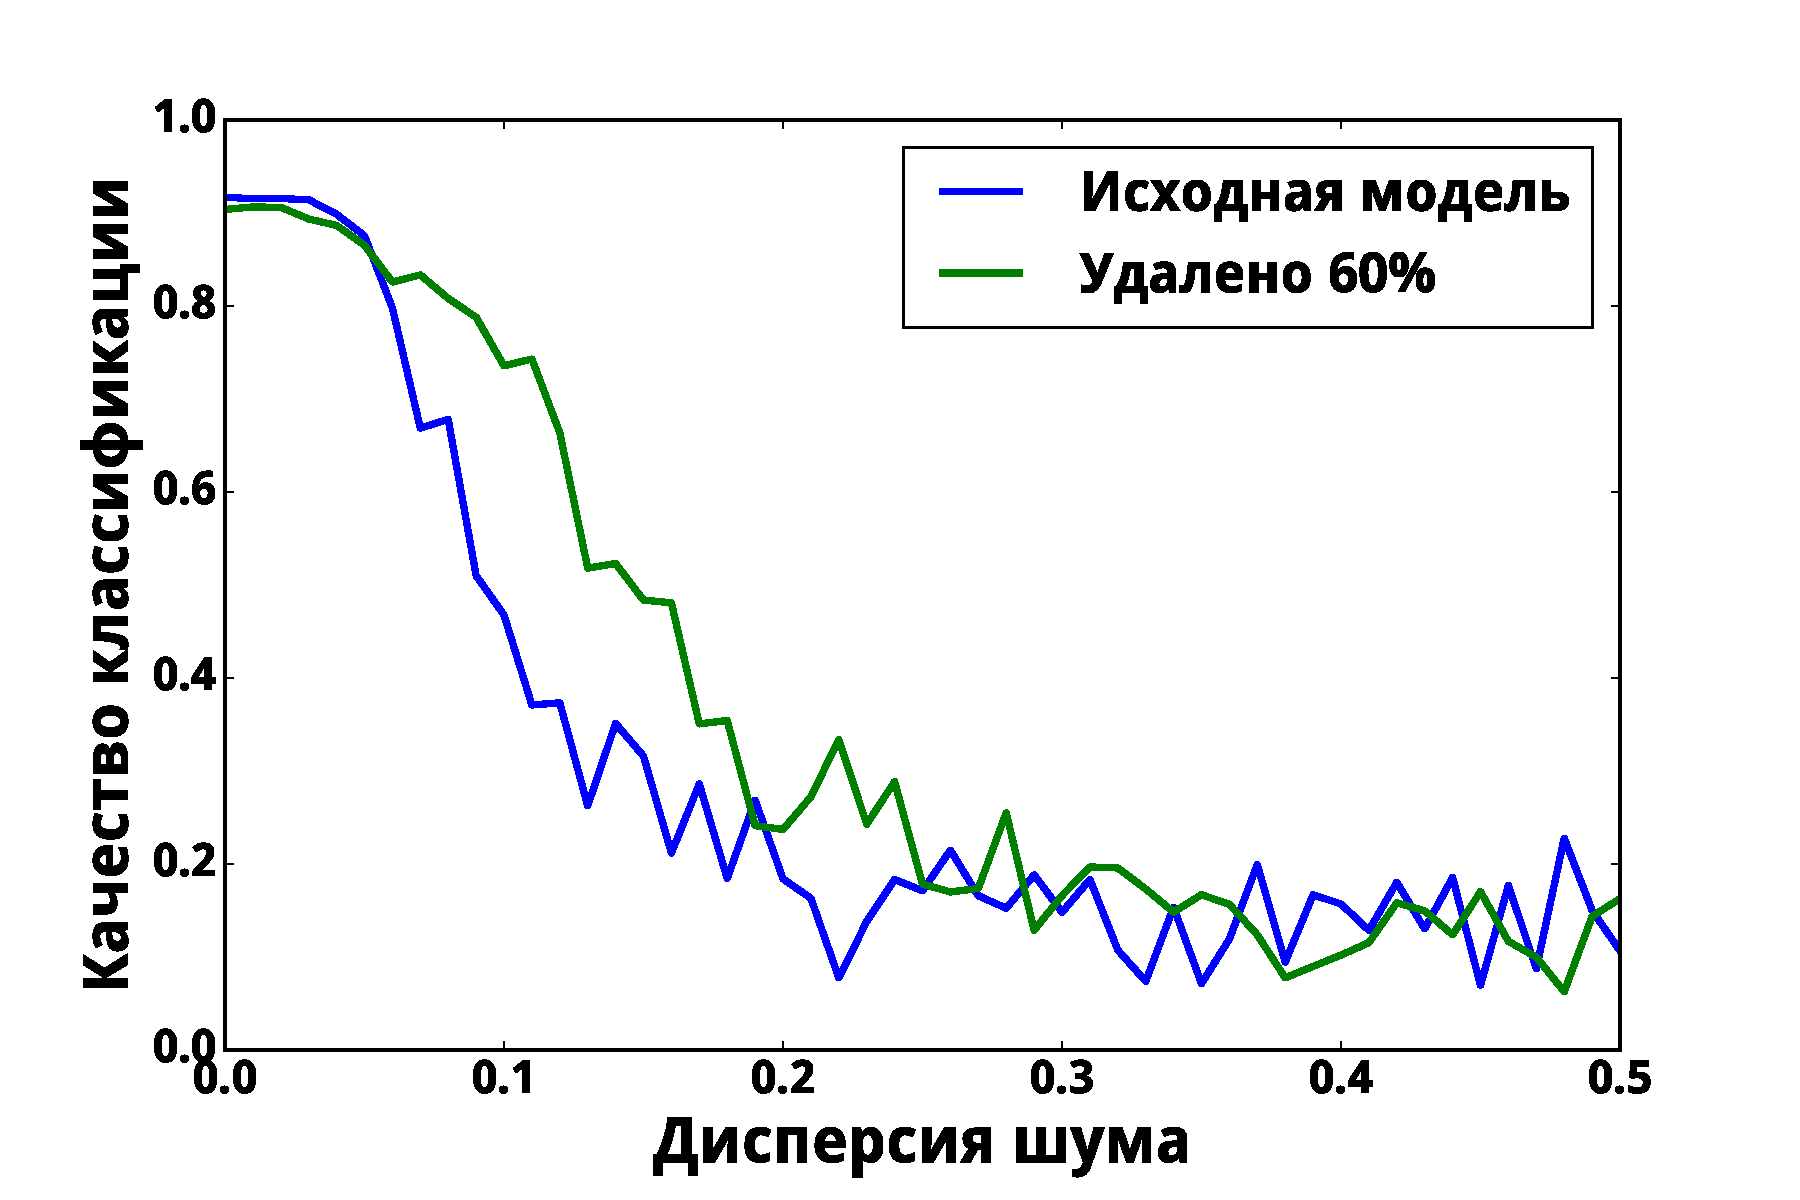
\includegraphics[width=0.4\textwidth]{noise.pdf}} 
 \subfloat[Качество классификации при удалении параметров]{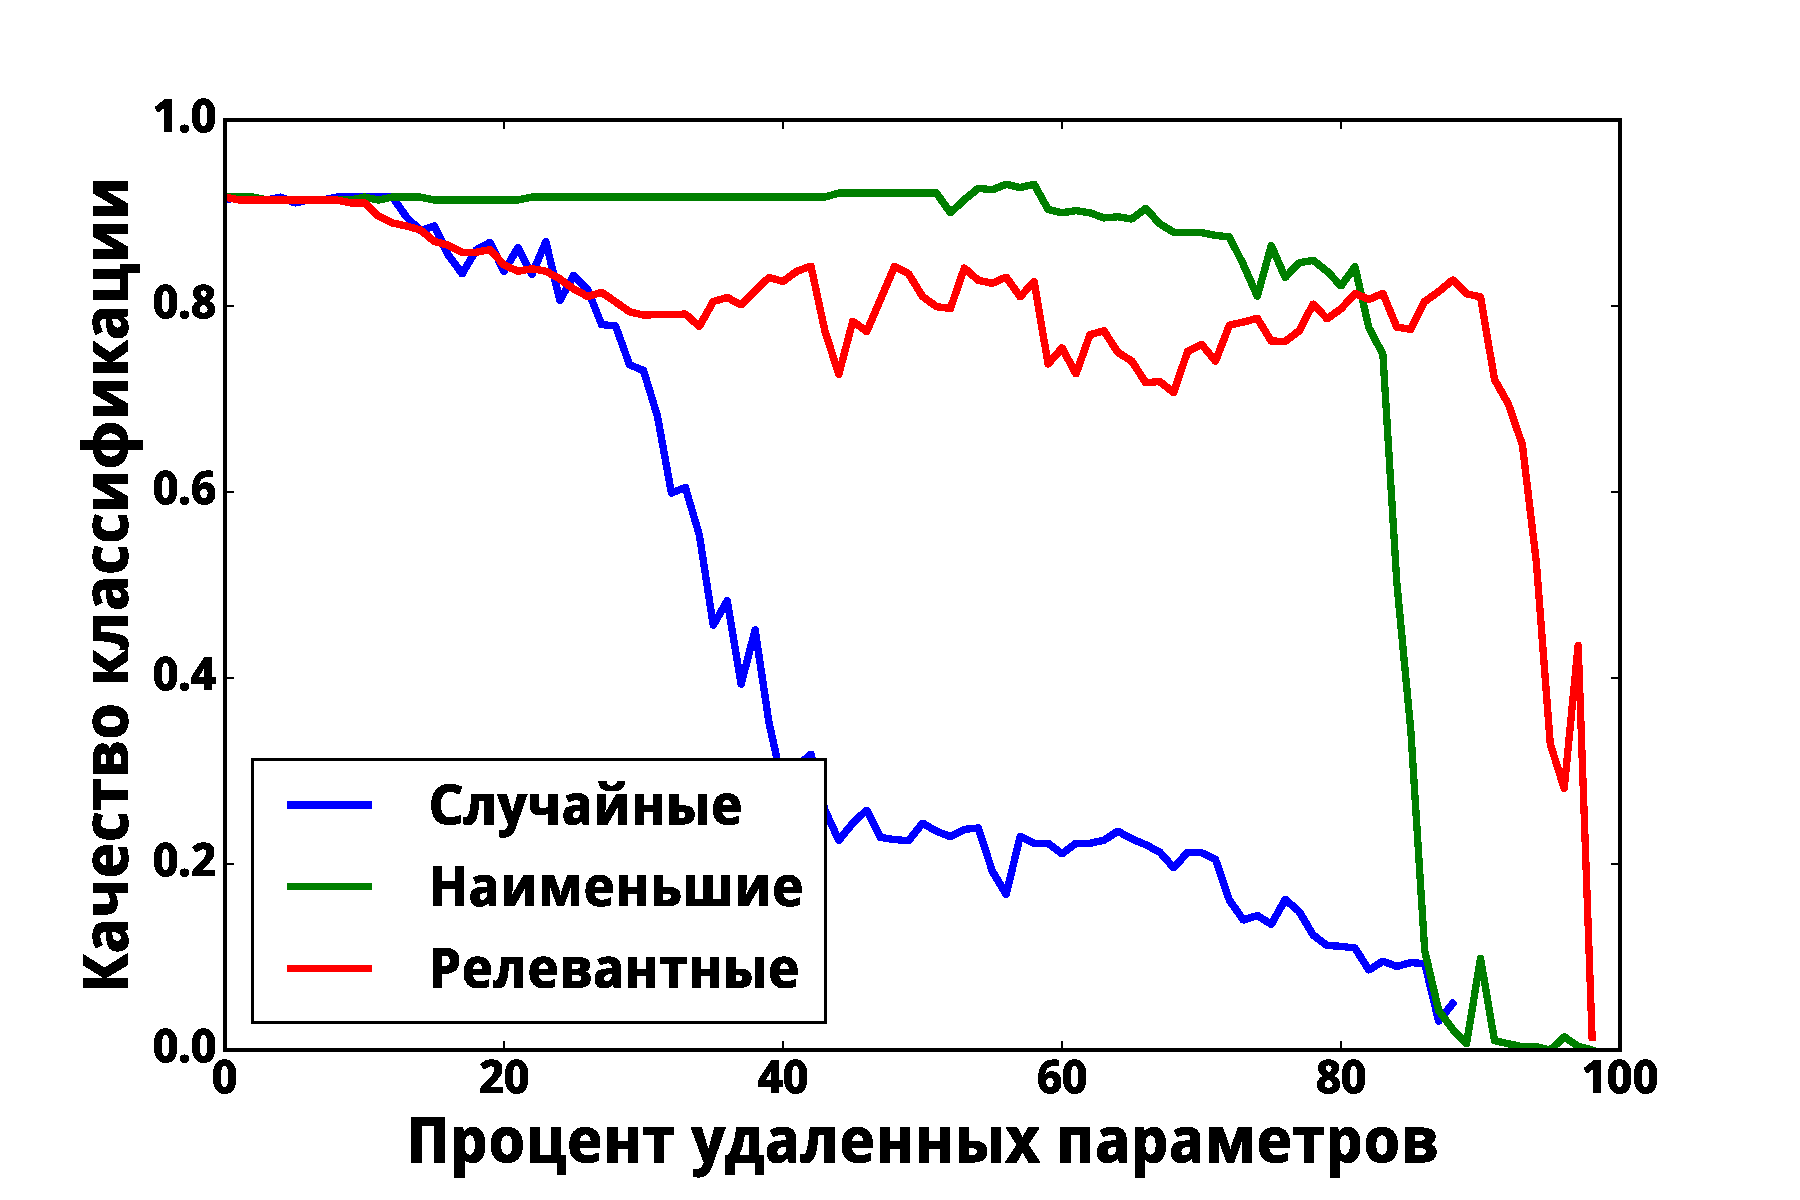
\includegraphics[width=0.4\textwidth]{pruning.pdf}}
\label{fig:1}\qquad

\end{figure}


\end{frame}

\begin{frame}{Сложность модели: зачем?}

\begin{figure}
  \centering
 {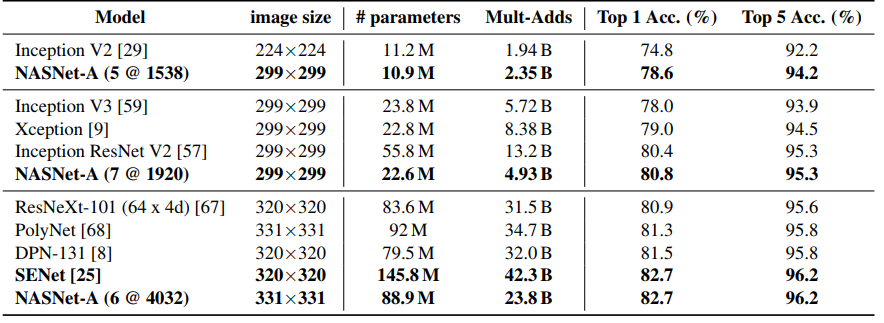
\includegraphics[width=\textwidth]{zoph.png}}
\label{fig:1}\qquad
\caption*{Zoph et al., 2017.  Сложность моделей отличается почти в два раза при одинаковом качестве.}
\end{figure}
\end{frame}

\begin{frame}{Устойчивость}
\begin{figure}
  \centering
 {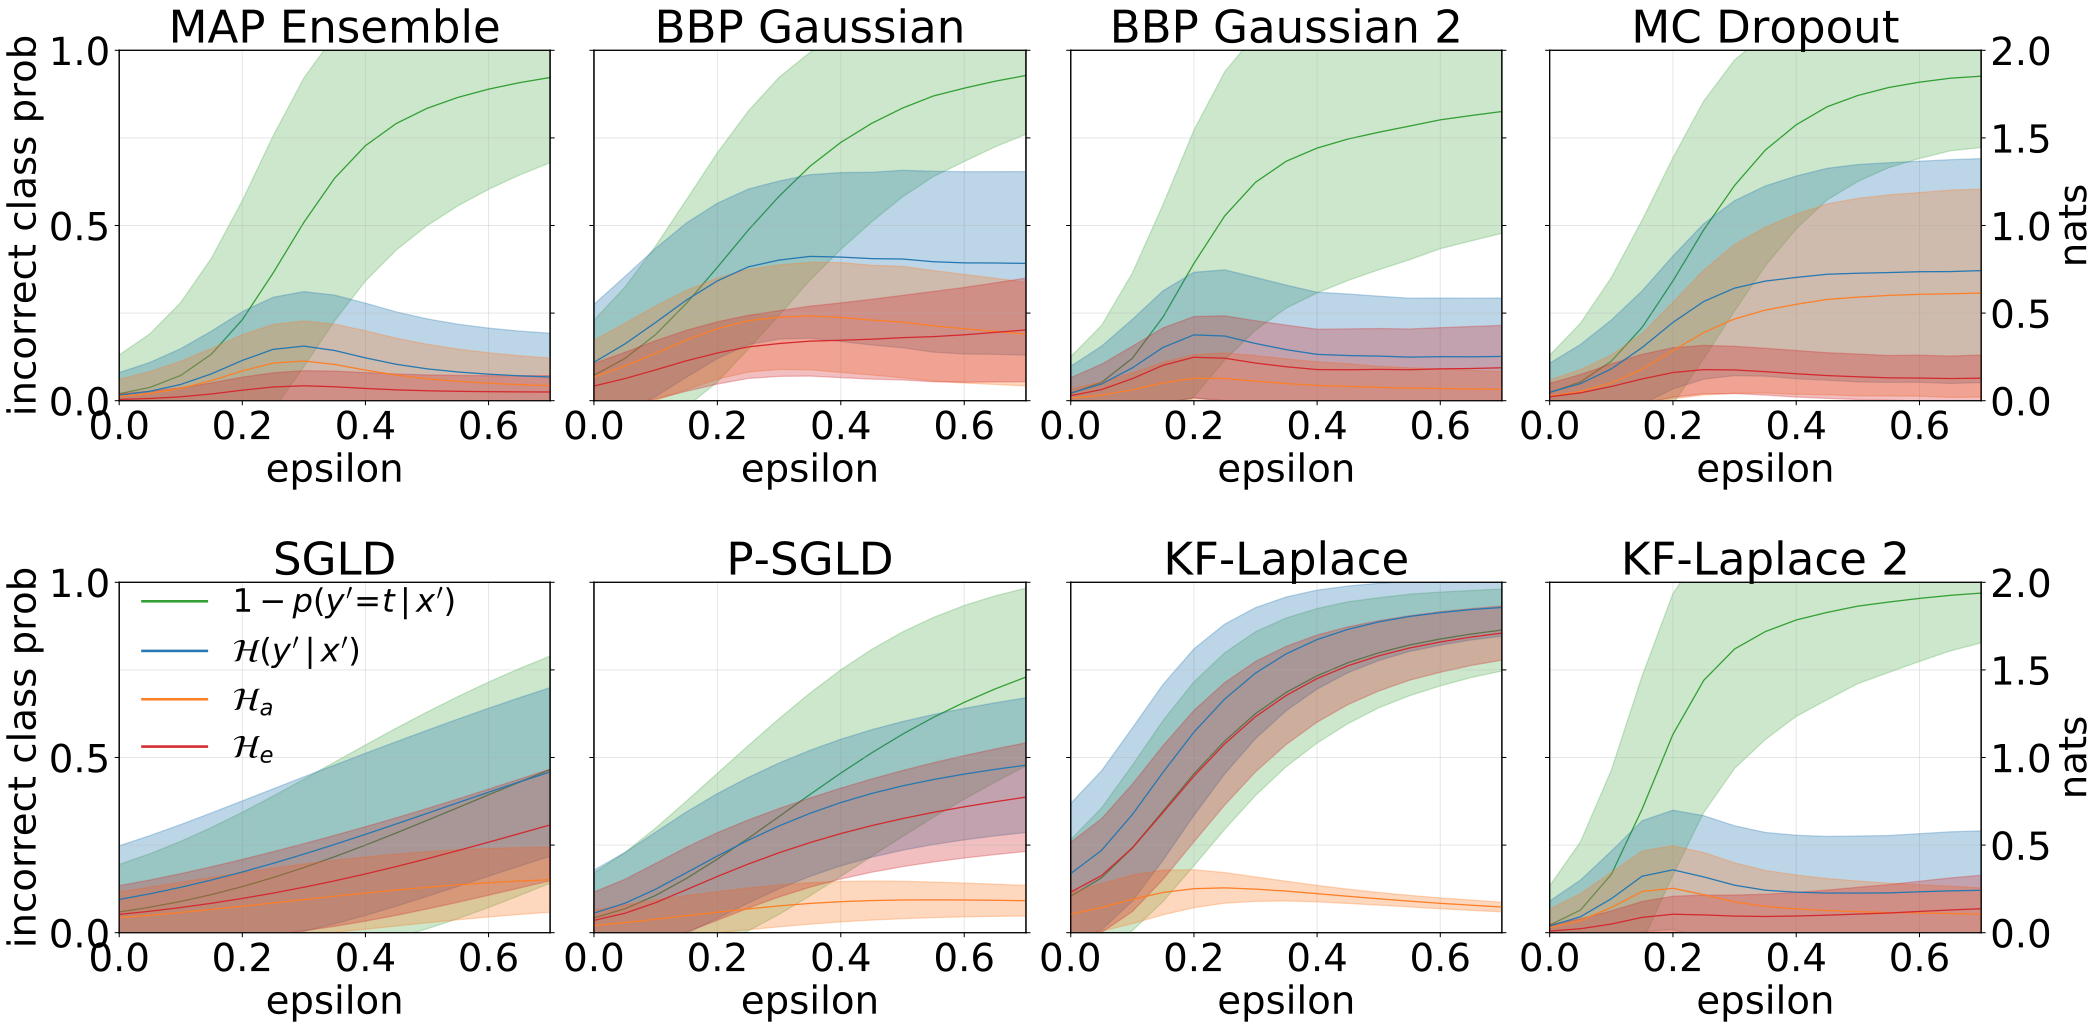
\includegraphics[width=\textwidth]{rotations.png}}
\label{fig:1}\qquad
\caption*{https://github.com/JavierAntoran/Bayesian-Neural-Networks}
\end{figure}

\end{frame}



\begin{frame}{Устойчивость}
\begin{figure}
  \centering
 {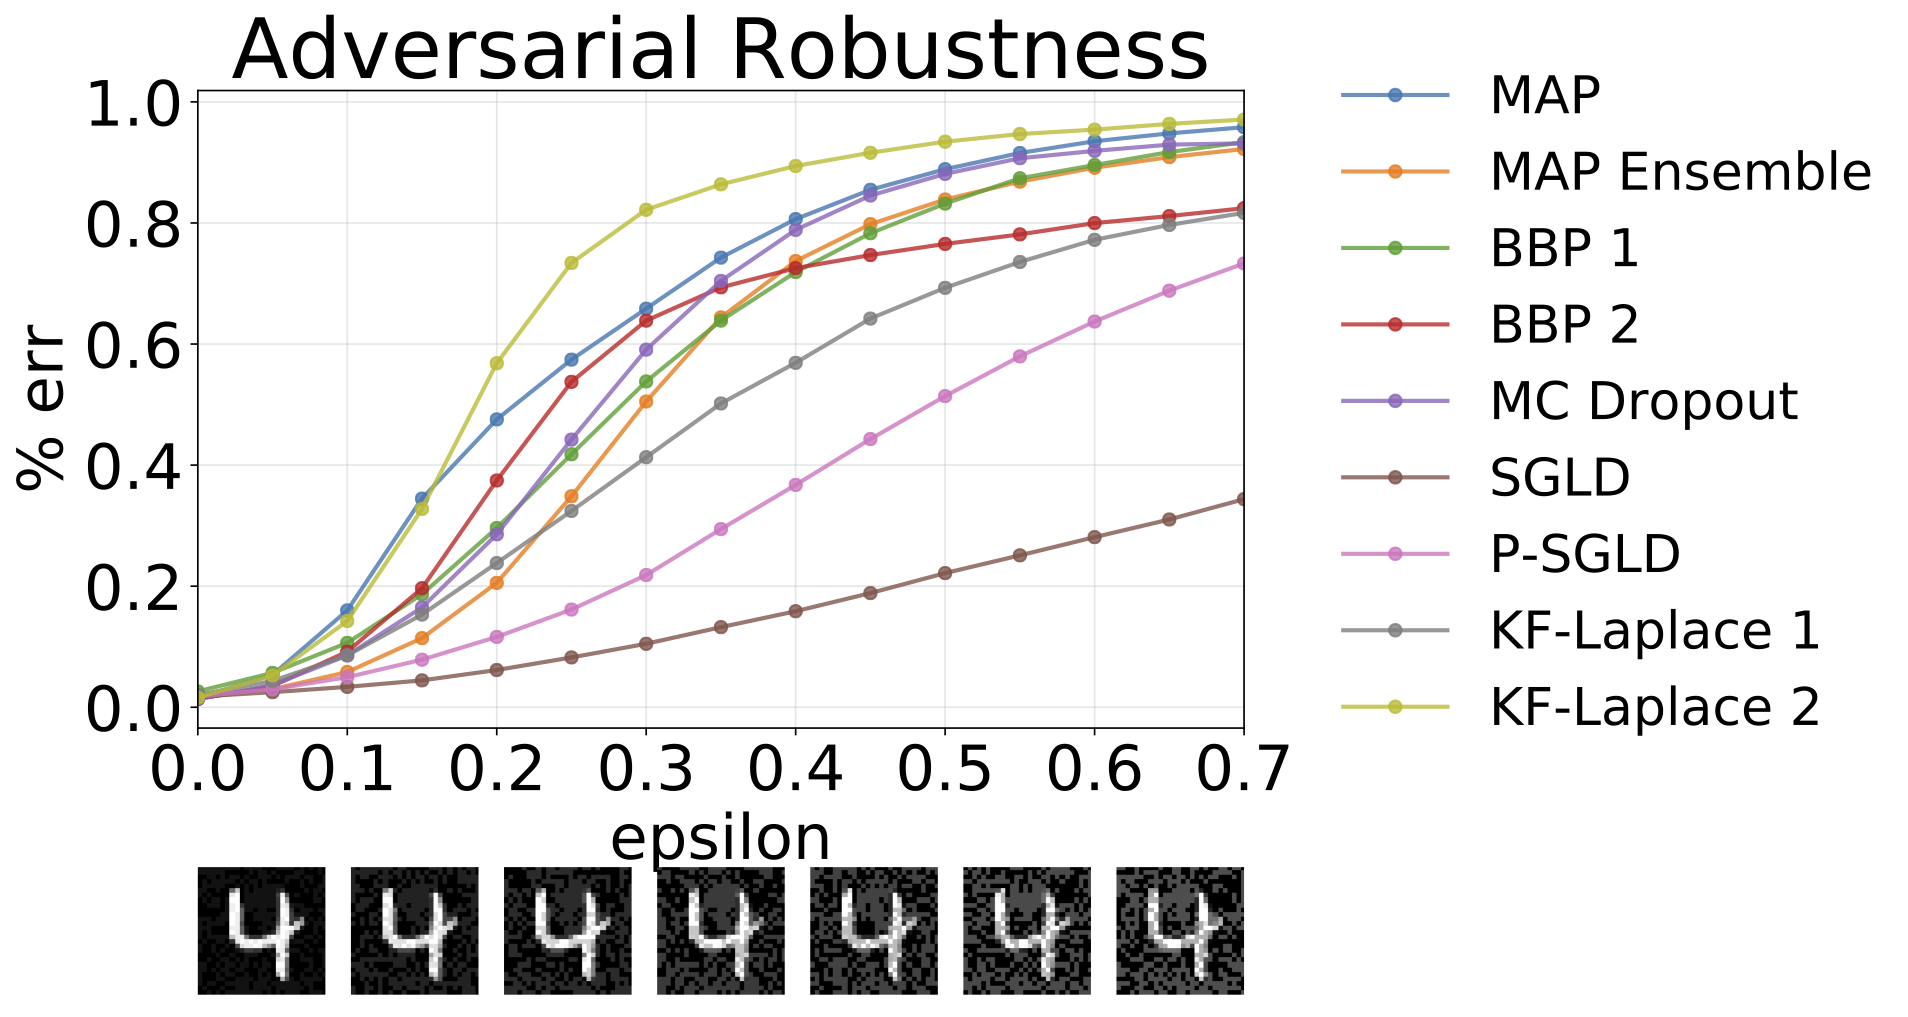
\includegraphics[width=\textwidth]{kf_laplace.png}}
\label{fig:1}\qquad
\caption*{https://github.com/JavierAntoran/Bayesian-Neural-Networks}
\end{figure}

\end{frame}

\begin{frame}{Связанный байесовский вывод}
\textit{Первый уровень:} выбираем оптимальные параметры:
\[
    \mathbf{w} = \argmax \frac{p(\mathfrak{D}|\mathbf{w})p(\mathbf{w}|\mathbf{h})}{p(\mathfrak{D}|\mathbf{h})},
\]

\textit{Второй уровень:} выбираем модель, доставляющую максимум обоснованности модели.

Обоснованность модели (``Evidence''):
\[
	p(\mathfrak{D}|\mathbf{h}) = \int_\mathbf{w} \textcolor{blue}{p(\mathfrak{D}|\mathbf{w})}\textcolor{red}{p(\mathbf{w}|\mathbf{h})} d\mathbf{w}.
\]


\begin{figure}
  \centering
  \subfloat[Схема выбора модели]{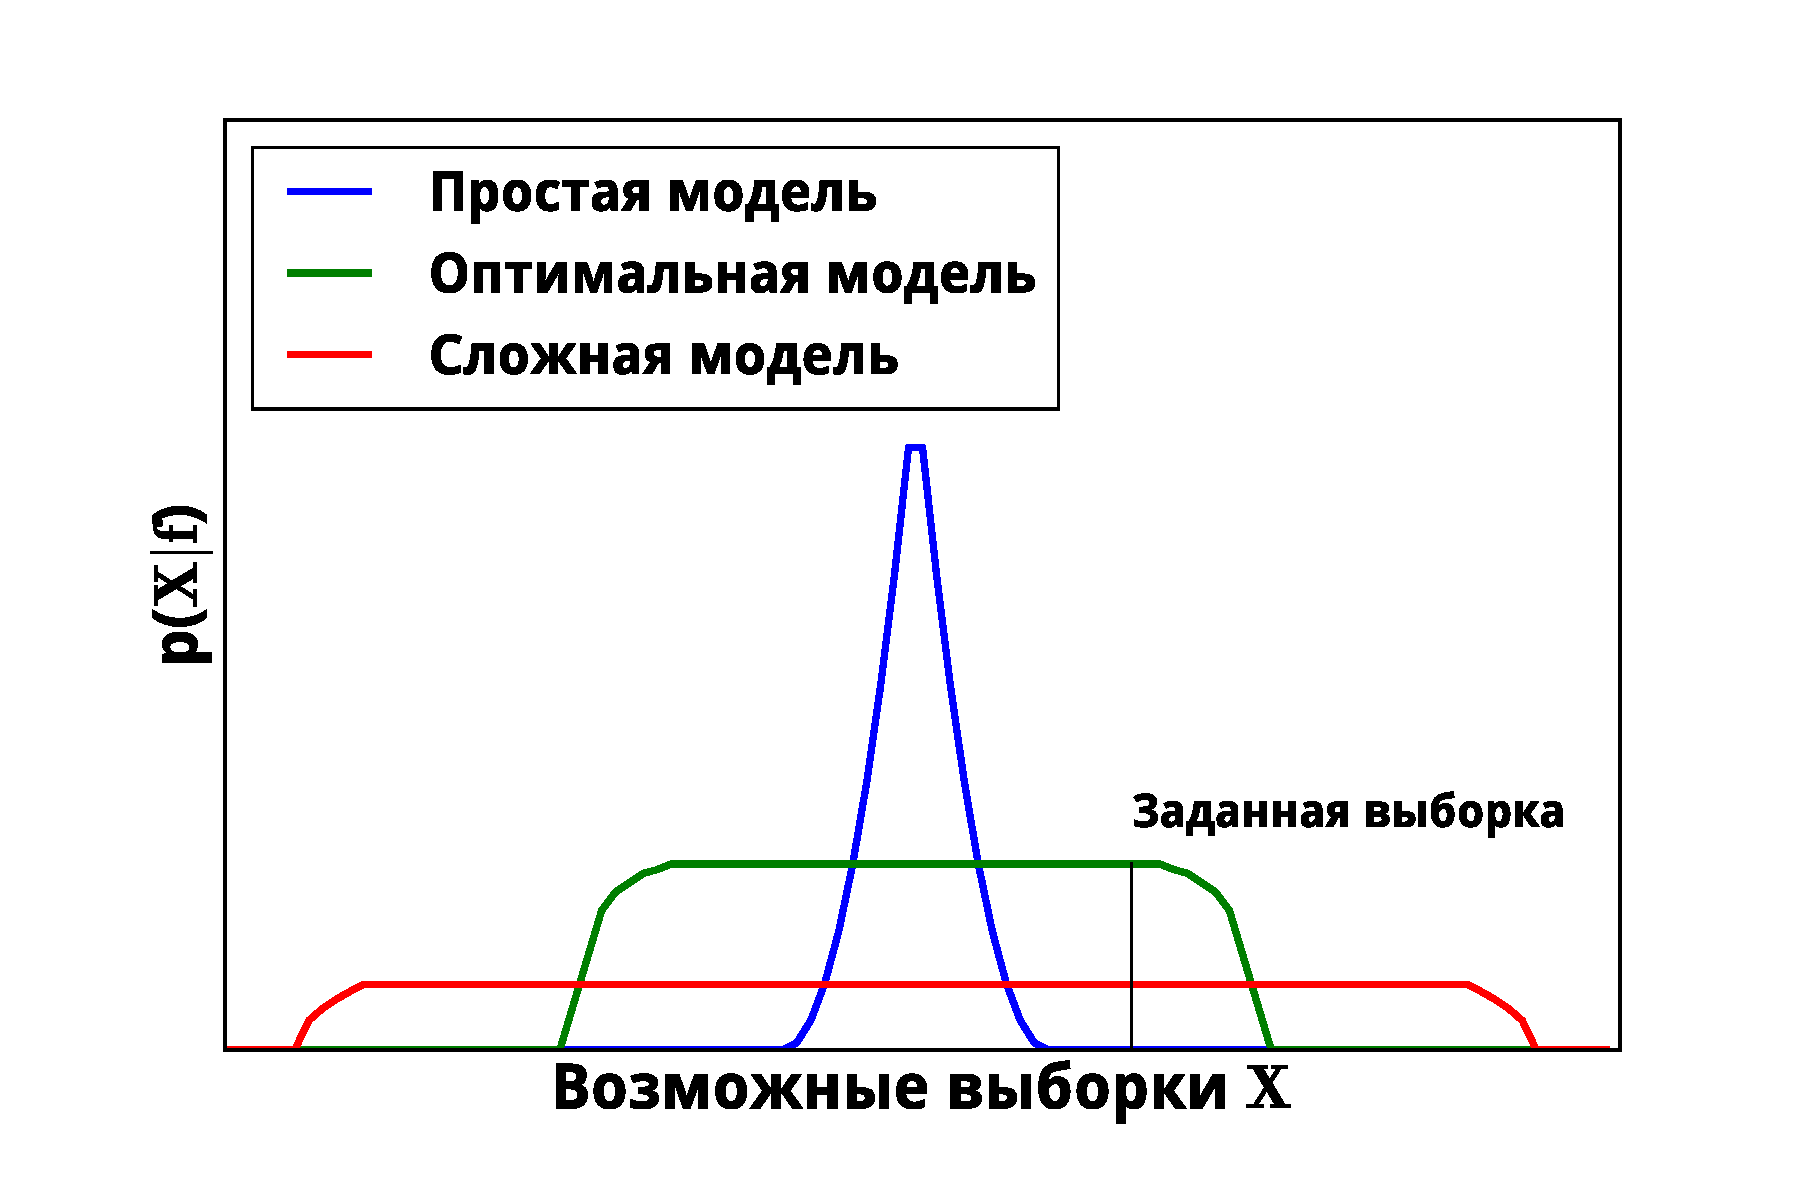
\includegraphics[width=0.4\textwidth]{evidence.pdf}} 
 \subfloat[Пример: полиномы]{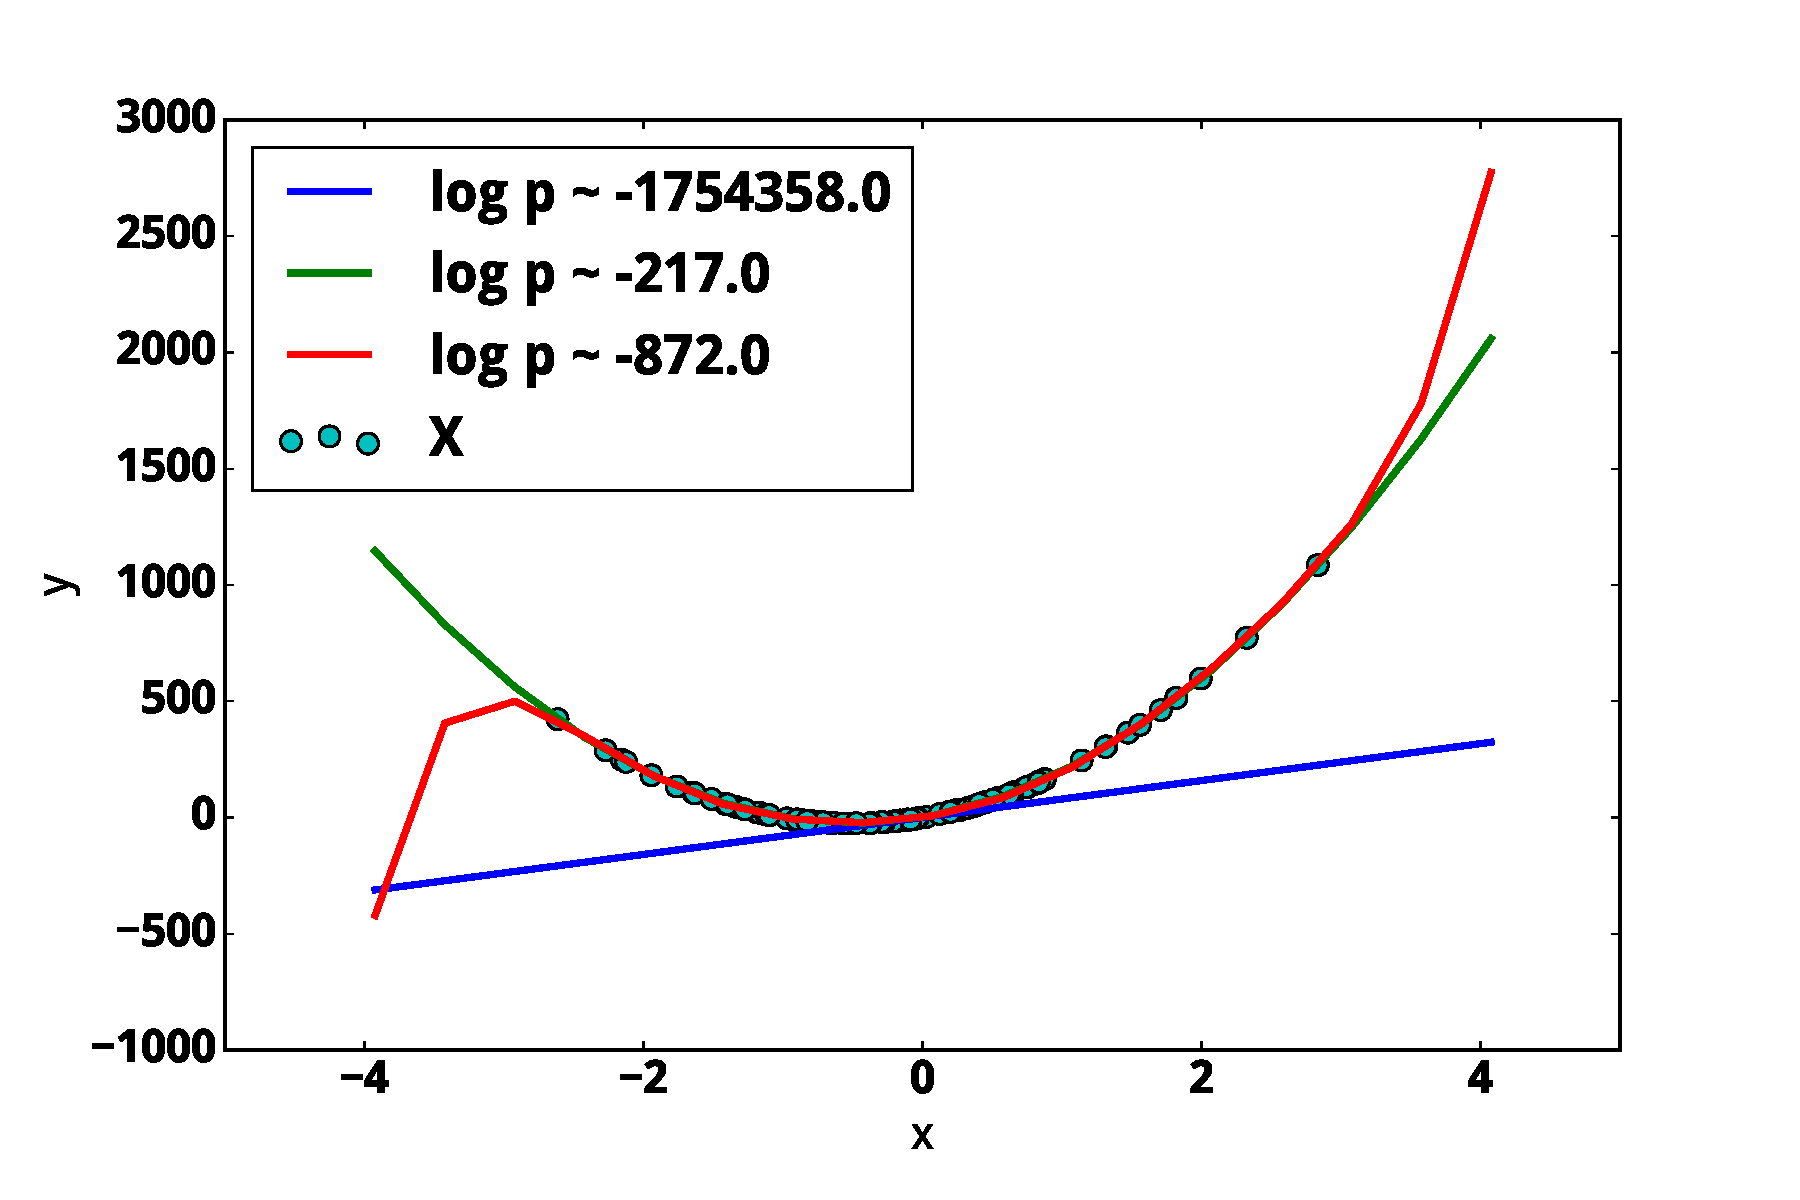
\includegraphics[width=0.4\textwidth]{example.pdf}}
\label{fig:1}\qquad

\end{figure}

\end{frame}



\begin{frame}{Принцип минимальной длины описания}
\[
\text{MDL}(\mathbf{f}, \mathfrak{D}) = L(\mathbf{f}) + L(\mathfrak{D}|\mathbf{f}),
\]
где $\mathbf{f}$ --- модель, $\mathfrak{D}$ --- выборка, $L$ --- длина описания в битах.
\\
\[
\text{MDL}(\mathbf{f}, \mathfrak{D}) \sim L(\mathbf{f}) + \textcolor{blue}{L(\mathbf{w}^*| \mathbf{f})} + \textcolor{red}{L(\mathfrak{D}|\mathbf{w}^*, \mathbf{f})},
\]
$\mathbf{w}^*$ --- оптимальные параметры модели.\\

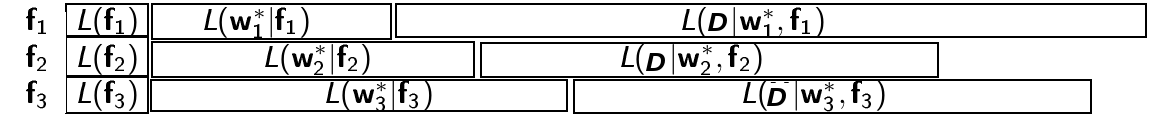
\includegraphics[width=\textwidth]{./mdl.png}

\end{frame}

\begin{frame}{MDL и Колмогоровская сложность}
\textbf{Колмогоровская сложность} --- длина минимального кода для выборки на предварительно заданном языке.

\textbf{Теорема инвариантности}\\
Для двух сводимых по Тьюрингу языков колмогоровская сложность  отличается не более чем на константу, не зависяющую от мощности выборки.\\

\textbf{Отличия от MDL}:
\begin{itemize}
\item Колмогоровская сложность невычислима.
\item Длина кода может зависеть от выбранного языка. Для небольших выборок теорема инвариантности не дает адекватных результатов.
\end{itemize}
\end{frame}

\begin{frame}{Evidence vs MDL}
\small
\begin{tabular}{ c | c  }
  \hline			
 \bf Evidence & \bf MDL \\
  \hline  
Использует априорные знания &  Независима от априорных знаний \\
  \hline  
Основывается на гипотезе о порождении\\ выборки & Минимизирует длину описания выборки\\ вне зависимости от их природы \\
  \hline  

\end{tabular}
\end{frame}



\section{Вариационная нижняя оценка}
\begin{frame}{Вариационная оценка, ELBO}
%http://www.orchid.ac.uk/eprints/40/1/fox_vbtut.pdf
\textbf{Вариационная оценка Evidence}, Evidence lower bound --- метод нахождения приближенного значения аналитически невычислимого распределения $p(\mathbf{w}|\mathfrak{D}, \mathbf{h})$ распределением $q(\mathbf{w}) \in \mathfrak{Q}$. Получение вариационной нижней оценки обычно сводится к задаче минимизации
$$\text{KL}(q(\mathbf{w})||p(\mathbf{w}| \mathfrak{D}))=
-\int_{\mathbf{w}} q(\mathbf{w}) \text{log}~\frac{p(\mathbf{w}| \mathfrak{D})} {q(\mathbf{w})}d\mathbf{w} = \textcolor{blue}{\mathsf{E}_{\mathbf{w}} \text{log}~p(\mathfrak{D}|\mathbf{w})} - \textcolor{red}{\text{KL}(q(\mathbf{w})||p(\mathbf{w}| \mathbf{h}))}.
$$

\begin{figure}
  \centering
  \subfloat[Вариационный вывод и expectation propogation (Bishop)]{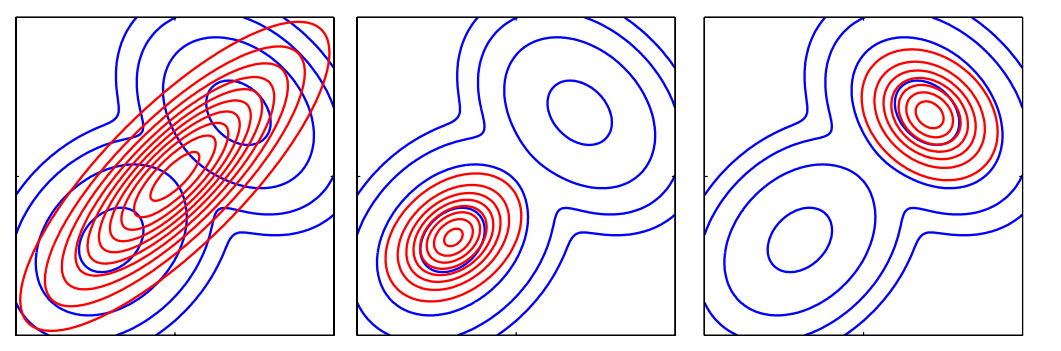
\includegraphics[width=0.66\textwidth]{bishop.png}} 
 \subfloat[{Аппроксимация Лапласа} и {вариационная оценка, зеленая линия}  (Bishop)]{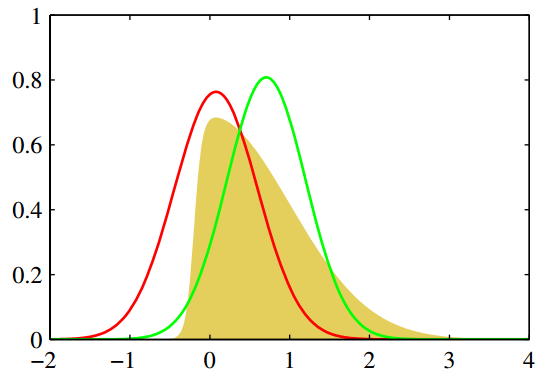
\includegraphics[width=0.33\textwidth]{laplace_vs_var.png}}
\label{fig:1}\qquad

\end{figure}

\end{frame}





\begin{frame}{ELBO: нормальное распределение}
\begin{columns}[T] 
\begin{column}{.48\textwidth}
\textbf{``Обычная'' функция потерь:}\\
$$
L = \textcolor{blue}{\sum_{\mathbf{x}, \mathbf{y} \in \mathfrak{D}} - \text{log}p(\mathbf{y}|\mathbf{x}, \mathbf{w})} + \textcolor{red}{\lambda||\mathbf{w}||_2^2}.
$$\\~\\

% если n - константна.
\textbf{Вариационный вывод при $(p(\mathbf{w}|\mathbf{h}) \sim \mathcal{N}(\mathbf{0}, \mathbf{1}))$:}\\
$$
L =   \textcolor{blue}{\sum_{\mathbf{x}, \mathbf{y}} \text{log}~p(\mathbf{y}|\mathbf{x}, \hat{\mathbf{w}})} +
$$
$$ + \textcolor{red}{\frac{1}{2} \bigl( \text{tr} (\mathbf{A}_q) + \boldsymbol{\mu}_q^\text{T}\mathbf{A}^{-1}\boldsymbol{\mu}_q  - \text{ln}~|\mathbf{A}_q| \bigr)}.
$$\\~\\

\end{column}%
\hfill%
\begin{column}{.48\textwidth}

\begin{center}
\begin{figure}
\caption*{Пример грубой аппроксимации нормальным диагональным распределением $q$}
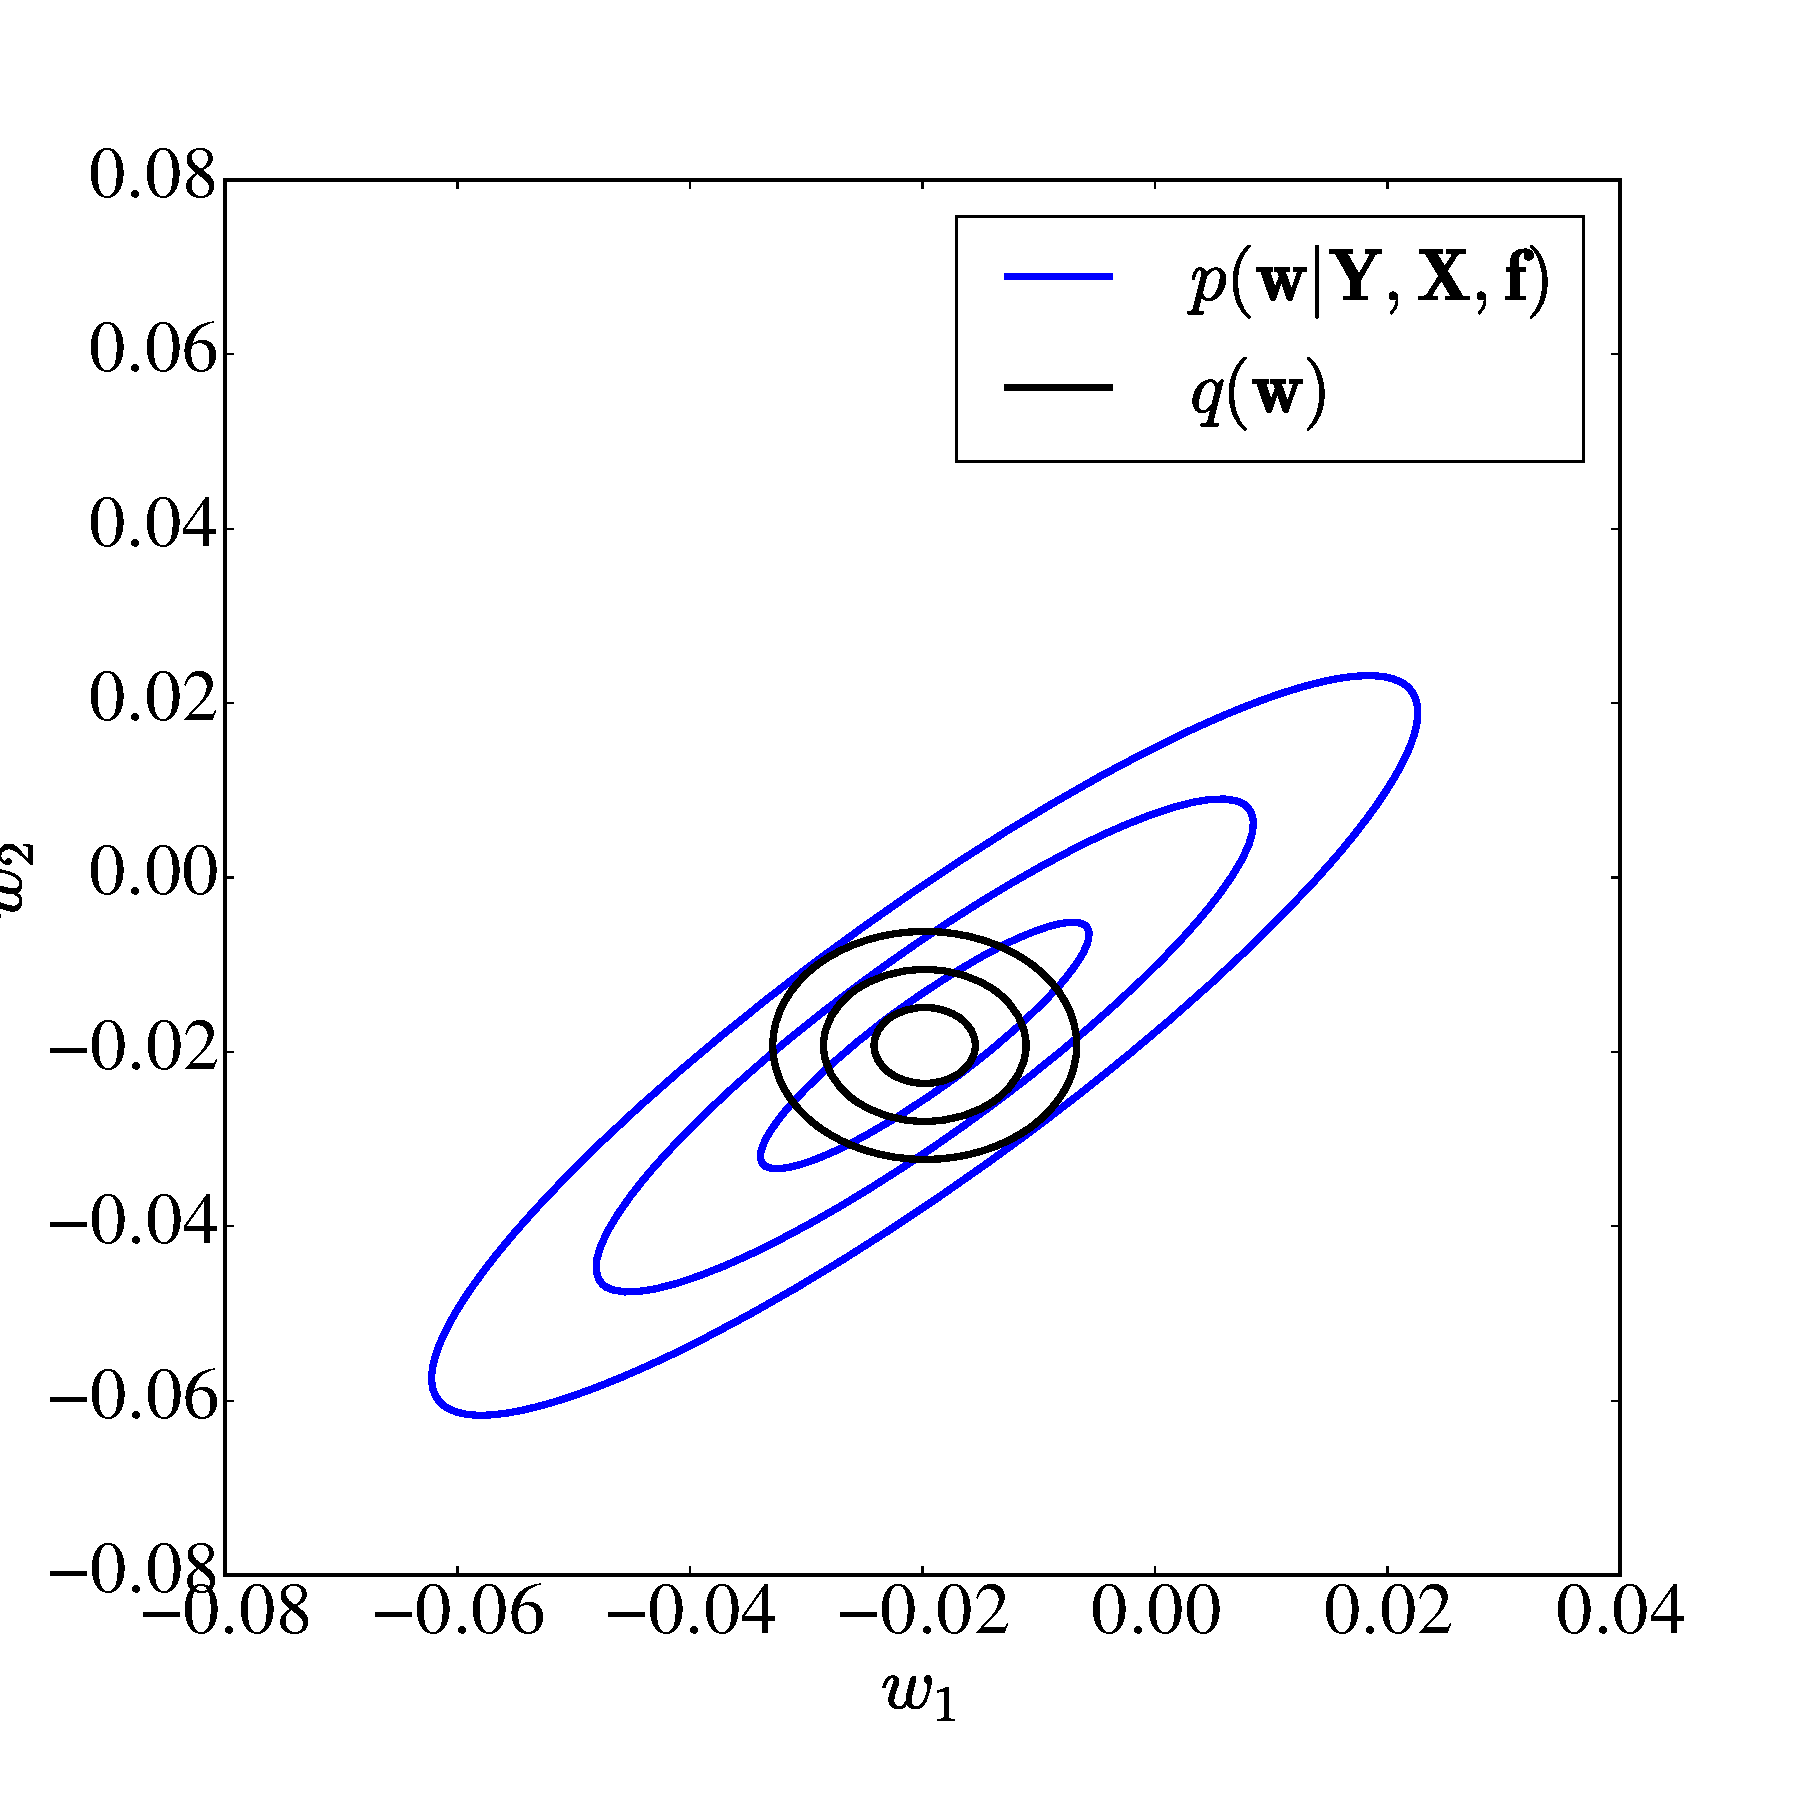
\includegraphics[width=0.8\textwidth]{mf.pdf}
\end{figure}
\end{center}

\end{column}%
\end{columns}

\end{frame}




\begin{frame}{Двухуровневая задача оптимизации}
\[
\mathbf{h}^{*} = \argmax_{\mathbf{h}} Q = 
\]
\[
= \textcolor{blue}{\lamLL\mathsf{E}_{\q[\teta^{*}]} \text{log}~{p(\mathbf{y} | \mathbf{X}, \mathbf{w}, \mathbf{h})}}
 -\]
\vspace{-0.3cm}
\[- \textcolor{red}{^\text{prior}_\text{Q}\text{D}_{KL}\bigl(\q[\teta^{*}] || p_1(\mathbf{w} |\mathbf{h}) \bigr)},\]
где 
\[
\teta^{*} = \argmax_{\teta} L = 
\textcolor{blue}{\mathsf{E}_q \text{log}~{p(\mathbf{y} | \mathbf{X}, \mathbf{w}, \mathbf{h})}}
\]
\vspace{-0.3cm}
\[- \textcolor{red}{^\text{prior}_\text{L}\text{D}_{KL}\bigl( q^{*}(\mathbf{w}) || p_2(\mathbf{w} |\mathbf{h}) \bigr)}.
\]

\end{frame}

\begin{frame}{Пример}
\[
\mathbf{h}^{*} = \argmax_{\mathbf{h}} Q = 
\]
\[
= \textcolor{blue}{\lamLL\mathsf{E}_{\q[\teta^{*}]} \text{log}~{p(\mathbf{y} | \mathbf{X}, \mathbf{w}, \mathbf{h})}}
 -\]
\vspace{-0.3cm}
\[- \textcolor{red}{^\text{prior}_\text{Q}\text{D}_{KL}\bigl(\q[\teta^{*}] || p_1(\mathbf{w} |\mathbf{h}) \bigr)},\]
где 
\[
\teta^{*} = \argmax_{\teta} L = 
\textcolor{blue}{\mathsf{E}_q \text{log}~{p(\mathbf{y} | \mathbf{X}, \mathbf{w}, \mathbf{h})}}
\]
\vspace{-0.3cm}
\[- \textcolor{red}{^\text{prior}_\text{L}\text{D}_{KL}\bigl( q^{*}(\mathbf{w}) || p_2(\mathbf{w} |\mathbf{h}) \bigr)}.
\]
Что будет, если $p_1 \neq p_2?$.
\begin{itemize}
\item $p_1 = p_2 \sim  \mathcal{N}(0, \mathbf{A}^{-1}):$ задача оптимизации обоснованности. Сводится к одноуровневой.
\item $p_1 \sim \mathcal{U}, p_2 \sim \mathcal{N}(0, \mathbf{A}^{-1})$: параметры доставляют максимум обоснованности, матрица $\mathbf{A}$ доставляет максимум правдоподобия. 
\end{itemize}

\end{frame}

\begin{frame}{Integrate vs maximize [MacKay]}
Два подхода к назначению гиперпараметров и оптимизации параметров:
\begin{itemize}
\item $\mathbf{h} = \argmax \int_{\mathbf{w}} p(\mathfrak{D}|\mathbf{w})p(\mathbf{w}|\mathbf{h})d\mathbf{w}.$
\item $\mathbf{w} =  \argmax \int_{\mathbf{w}'} p(\mathfrak{D}|\mathbf{w}')p(\mathbf{w}')d\mathbf{w}', \quad p(\mathbf{w}') = \int_{\mathbf{h}} p(\mathbf{w}'|\mathbf{h})d\mathbf{h}.$ 
\end{itemize}
\end{frame}

\begin{frame}{Informative prior vs Uninformative prior}
\begin{itemize}
\item Informative prior: соответствует экспертным знаниям о наблюдаемой переменной 
\begin{itemize}
\item Пример: температура воздуха: нормальная величина с известным средним и дисперсией, соответствующими прошлым наблюдениям.
\item Соответствие апостериорного распределения априорному назовем интерпретируемостью модели.
\item Ошибка в указании информативного априорного распределения может значительно снизить итоговое качество модели.
\end{itemize}

\item Uninformative prior: соответствует базовым предположениям о распределении переменной
\begin{itemize}
\item Пример: температура воздуха: равномерное распределение (improper).
\end{itemize}

\item Weakly-informative prior: где-то по середине
\begin{itemize}
\item Пример: температура воздуха: равномерное распределение от -50 до +50.
\end{itemize}


\end{itemize}
Вопрос: $\mathbf{w} \sim \mathcal{N}(0, \mathbf{A}^{-1})$ --- какой тип априорного распределения?


\end{frame}


\begin{frame}{Пример}
\[
\mathbf{h}^{*} = \argmax_{\mathbf{h}} Q = 
\]
\[
= \textcolor{blue}{\lamLL\mathsf{E}_{\q[\teta^{*}]} \text{log}~{p(\mathbf{y} | \mathbf{X}, \mathbf{w}, \mathbf{h})}}
 -\]
\vspace{-0.3cm}
\[- \textcolor{red}{^\text{prior}_\text{Q}\text{D}_{KL}\bigl(\q[\teta^{*}] || p_1(\mathbf{w} |\mathbf{h}) \bigr)},\]
где 
\[
\teta^{*} = \argmax_{\teta} L = 
\textcolor{blue}{\mathsf{E}_q \text{log}~{p(\mathbf{y} | \mathbf{X}, \mathbf{w}, \mathbf{h})}}
\]
\vspace{-0.3cm}
\[- \textcolor{red}{^\text{prior}_\text{L}\text{D}_{KL}\bigl( q^{*}(\mathbf{w}) || p_2(\mathbf{w} |\mathbf{h}) \bigr)}.
\]
\textbf{Гипотеза}\\
Что будет, если $p_1 \neq p_2?$.
\begin{itemize}
\item $p_1 = p_2 = \text{informative}: $задача оптимизации обоснованности. Сводится к одноуровневой. Может вести к переобучению.
\item $p_1 = \text{informative}; p_2 =\text{uninformative}.$ компромисс между информативностью и неинформативностью модели.
\end{itemize}

\end{frame}






\begin{frame}{Базовые методы оптимизации гиперпараметров}
Варианты:
\begin{itemize}
\item Поиск по решетке;
\item Случайный поиск.
\end{itemize}

Оба метода страдают от проклятия размерности.

Случайный поиск может быть более эффективным, если пространство гиперпараметров вырождено.
\begin{figure}
\begin{centering}
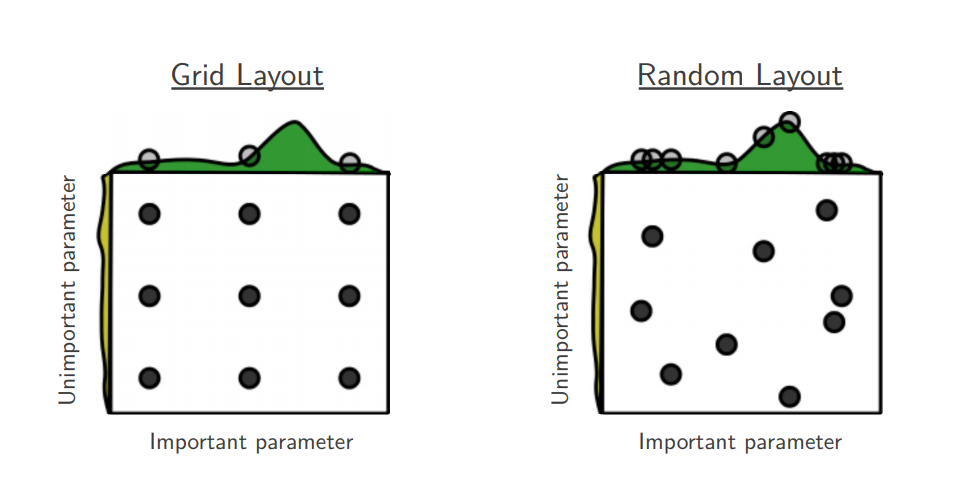
\includegraphics[width=0.5\textwidth]{random_search.png}
\end{centering}
\caption*{Bergstra et al., 2012}
\end{figure}
\end{frame}

\begin{frame}{Гауссовый процесс}

\begin{columns}
\begin{column}{0.5\textwidth}
\textbf{Идея:}

Будем моделировать $Q(\boldsymbol{\theta}(\mathbf{h})^{*}, \mathbf{h})$ гауссовым процессом, зависящим от $\mathbf{h}$.

~\\
\textbf{Плюсы:}
\begin{itemize}
\item Гибкость модели.
\item Дешевле, чем обучения модели.
\end{itemize}

~\\
\textbf{Минусы:} кубическая сложность по количеству гиперпараметров.

\end{column}
\begin{column}{0.4\textwidth}
\begin{figure}[h]
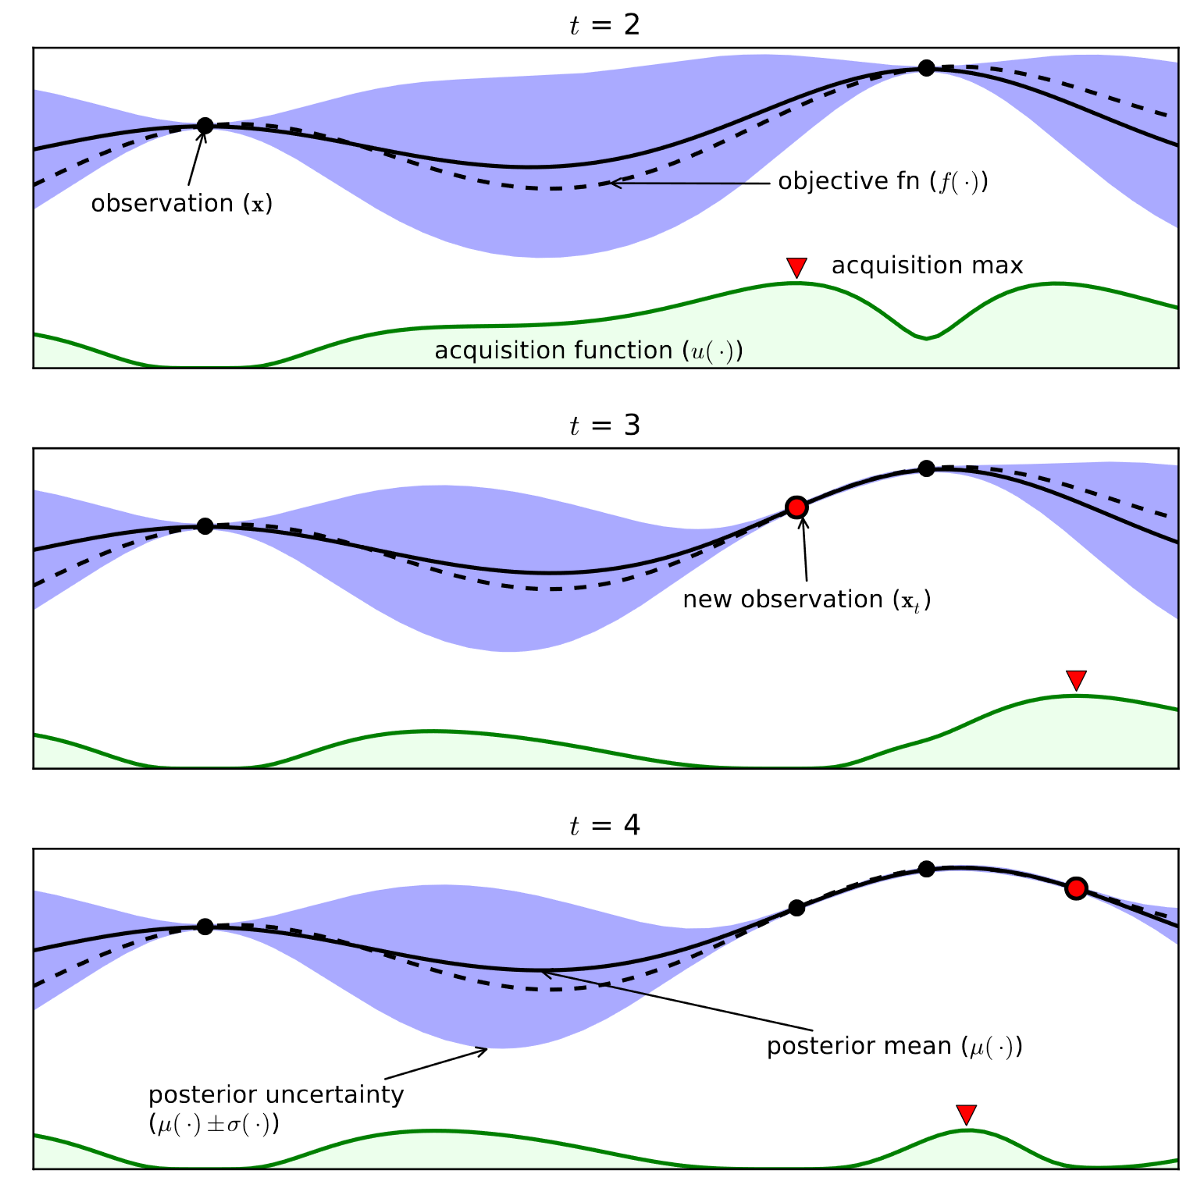
\includegraphics[width=\textwidth]{./gp.png}
\caption*{Shahriari et. al, 2016. Пример работы гауссового процесса.}
\end{figure}

\end{column}
\end{columns}
\end{frame}


\begin{frame}{Градиентные методы}
\begin{columns}
\begin{column}{0.5\textwidth}
\textbf{Идея:}
Будем производить оптимизацию вдоль всей траектории оптимизации параметров.

\textbf{Плюсы:}
\begin{itemize}
\item Оптимизация гиперпараметров будет учитывать оптимизацию параметров.
\item Сложность меняется незначительно от количества гиперпараметров.
\end{itemize}

~\\
\textbf{Минусы:} вычилсительно дорого.

\end{column}
\begin{column}{0.4\textwidth}
\begin{figure}[h]
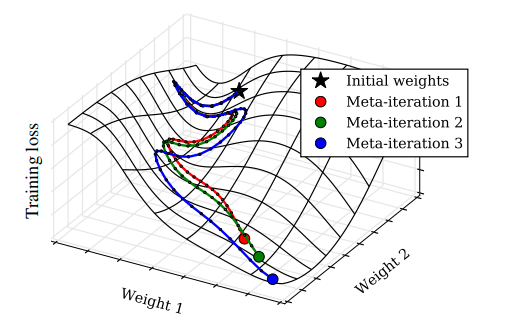
\includegraphics[width=\textwidth]{./grad.png}
\caption*{Maclaurin et. al, 2015. Пример работы.}
\end{figure}

\end{column}
\end{columns}

\end{frame}



\begin{frame}{Аналитическая формула оптимизации параметров}
\begin{block}{Утверждение (Pedregosa, 2016)}
Пусть $L$ --- дифференцируемая выпуклая функция.
Пусть также гессиан $\mathbf{H}^{-1}$ функции потерь $L$ является обратимым в каждой стационарной точке.\\
Тогда
\[
\nabla_{\mathbf{h}}Q(T(\boldsymbol{\theta}_0, \mathbf{h}), \mathbf{h}) =  \nabla_{\mathbf{h}}Q(\boldsymbol{\theta}^\eta, \mathbf{h}) - \nabla_{\mathbf{h}}\nabla_{\boldsymbol{\theta}} L(\boldsymbol{\theta}^\eta, \mathbf{h})^\text{T}\mathbf{H}^{-1}\nabla_{\boldsymbol{\theta}}Q(\boldsymbol{\theta}^\eta, \mathbf{h}).
\]
\end{block}

\end{frame}


\begin{frame}{Жадная оптимизация гиперпараметров}
На каждом шаге оптимизации параметров $\boldsymbol{\theta}$:
\[
	\mathbf{h}' = \mathbf{h} - \beta_{\mathbf{h}} \nabla_{\mathbf{h}}  Q \bigl(T(\boldsymbol{\theta}, \mathbf{h}) , \mathbf{h}\bigr) = \mathbf{h} - \beta_{\mathbf{h}} \nabla_{\mathbf{h}}  Q\bigl(\boldsymbol{\theta} - \beta \nabla L(\boldsymbol{\theta}, \mathbf{h}), \mathbf{h})\bigr),
\]
где $\beta_{\mathbf{h}}$ --- длина шага оптимизации гиперпараметров.

Метод является приближением к решению аналитической формуле в случае $\mathbf{H}^{-1} \sim \mathbf{I}$.

\end{frame}


\begin{frame}{Параметрическая сложность}
Пусть задано неинформативное априорное распределение.
\begin{block}{Определение}
Параметрической сложностью модели назовем минимальную дивергенцию между априорным и вариационным распределением:
\vspace{-0.2cm}
\[
    C_p = \min_{\mathbf{h}} \textcolor{red}{D_\text{KL}(q||p(\mathbf{w}|\mathbf{h})).}
\]
\end{block}
\vspace{-0.2cm}

\begin{block}{Утвреждение}
Устремление $C_p$ к нулю эквивалентно снижению информативности всех параметров модели.
\end{block}
\end{frame}

\begin{frame}{Вариационная оценка и эффективный размер выборки}
\begin{block}{Утверждение 2}
Пусть $m \gg 0$, $\lambda > 0, \frac{m}{\lambda}   \in \mathbb{N}, \frac{m}{\lambda}  \gg 0.$ Тогда оптимизация функции
\[
\textcolor{blue}{\mathsf{E}_{q} \log p(\mathbf{y}|\mathbf{X}, \mathbf{w})} - \textcolor{red}{\lambda \textnormal{D}_\textnormal{KL}  \bigl(q(\mathbf{w})||p(\mathbf{w}|\mathbf{y}, \mathbf{X}, \mathbf{h})\bigr)}
\]
 эквивалентна оптимизации вариационной оценки обоснованности  
для произвольной случайной подвыборки $\hat{\mathbf{y}}, \hat{\mathbf{X}}$ мощности $\frac{m}{{\lambda}}$ из генеральной совокупности.
\end{block}

См. также [Alemi et al., 2017, Fixing Broken ELBO].
\end{frame}




\begin{frame}{Вывод}
\begin{itemize}
\item Чем больше коэффициент перед регуляризации модели, тем выше влияние априорного распределения.
\item Интерпретация отклонения от априорного распределения различается в зависимости от его характера:
\begin{itemize}
\item Неинформативное распределение: модель несет больше информации.
\item Информативное распределение: модель несет меньше информации (или априорное распределение установлено некорректно).
\end{itemize}
\end{itemize}
\end{frame}

\begin{frame}{Список источников}
\begin{itemize}
\item Zoph, B., Vasudevan, V., Shlens, J. and Le, Q.V., 2018. Learning transferable architectures for scalable image recognition
\item David J. C. MacKay, Information Theory, Inference \& Learning Algorithms
\item Peter Grunwald, A tutorial introduction to the minimum description length principle
\item Kuznetsov M.P., Tokmakova A.A., Strijov V.V. Analytic and stochastic methods of structure parameter estimation
\item Christopher Bishop, Pattern Recognition and Machine Learning
\item Diederik P Kingma, Max Welling, Auto-Encoding Variational Bayes
\item Dougal Maclaurin, David Duvenaud, Ryan P. Adams, Early Stopping is Nonparametric Variational Inference
\item Max Welling, Yee Whye Teh, Bayesian Learning via Stochastic Gradient Langevin Dynamics
\end{itemize}
\end{frame}

\begin{frame}
\frametitle{Список источников}
\begin{itemize}
\item A. Graves, Practical Variational Inference for Neural Networks
\item Salimans, Tim, Diederik Kingma, and Max Welling, 2015. Markov chain monte carlo and variational inference: Bridging the gap
\item Altieri: http://approximateinference.org/accepted/AltieriDuvenaud2015.pdf
\item Stephan Mandt, Matthew D. Hoffman, David M. Blei, 2017. Stochastic Gradient Descent as Approximate Bayesian Inference
\item О. Ю. Бахтеев, В. В. Стрижов, “Выбор моделей глубокого обучения субоптимальной сложности”
\item А. Н. Смердов, О. Ю. Бахтеев, В. В. Стрижов, “Выбор оптимальной модели рекуррентной сети в задачах поиска парафраза”
\end{itemize}
\end{frame}


\end{document}

